\documentclass[border=0pt]{standalone}
\usepackage{tikz}
\usetikzlibrary{decorations.pathreplacing,
  fadings,
  arrows,
  decorations.markings
}
\tikzset{>=latex}
\tikzfading[name=fade img right,left color=transparent!100, right color=transparent!0]
\tikzfading[name=fade img left,right color=transparent!100, left color=transparent!0]
\usepackage{graphicx}

\ifpdf
% Ensure reproducible output
\pdfinfoomitdate=1
\pdfsuppressptexinfo=-1
\pdftrailerid{}
\fi

\begin{document}
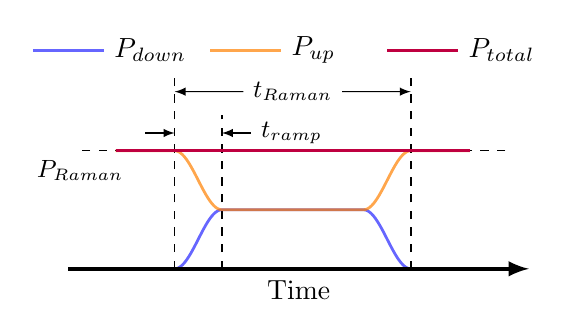
\begin{tikzpicture}[scale=1.5]
  % Legends
  \draw[line width=1,blue,opacity=0.6] (0.3, 1.85) -- ++(0.6, 0) node[right,black,opacity=1] {$P_{down}$};
  \draw[line width=1,orange,opacity=0.7] (1.8, 1.85) -- ++(0.6, 0) node[right,black,opacity=1] {$P_{up}$};
  \draw[line width=1,purple] (3.3, 1.85) -- ++(0.6, 0) node[right,black,opacity=1] {$P_{total}$};

  % Y (power) markers
  \draw[line width=0.5,dashed] (4.3, 1.0) -- (0.7, 1.0) node[below] {\small $P_{Raman}$};

  % X (time) markers
  \draw[line width=0.5,dashed] (1.5, 0) -- (1.5, 1.65);
  \draw[line width=0.5,dashed] (3.5, 0) -- (3.5, 1.65);
  \node (TRaman) at (2.5, 1.5) {\small $t_{Raman}$};
  \draw[->] (TRaman) -- (1.5, 1.5);
  \draw[->] (TRaman) -- (3.5, 1.5);

  \draw[line width=0.5,dashed] (1.9, 0) -- (1.9, 1.3);
  \draw[->] (1.25, 1.15) -- (1.5, 1.15);
  \draw[<-] (1.9, 1.15) -- (2.15, 1.15) node[right] {\small $t_{ramp}$};

  % Down leg
  \draw[line width=1,blue,opacity=0.6] (1.0, 0)
  -- plot[domain={-0.2}:{0.2},variable=\x] ({\x + 1.7}, {0.25*sin(180 * 5 / 2 * \x) + 0.25})
  -- (3.1, 0.5)
  -- plot[domain={-0.2}:{0.2},variable=\x] ({\x + 3.3}, {-0.25*sin(180 * 5 / 2 * \x) + 0.25})
  -- (4.0, 0);
  % Up leg
  \draw[line width=1,orange,opacity=0.7] (1.0, 1.0)
  -- plot[domain={-0.2}:{0.2},variable=\x] ({\x + 1.7}, {-0.25*sin(180 * 5 / 2 * \x) + 0.75})
  -- (3.1, 0.5)
  -- plot[domain={-0.2}:{0.2},variable=\x] ({\x + 3.3}, {0.25*sin(180 * 5 / 2 * \x) + 0.75})
  -- (4.0, 1.0);
  % Total
  \draw[line width=1,purple] (1.0, 1.0) -- (4.0, 1.0);
  \draw[line width=1.5,->] (0.6, 0) --  node[below] {Time} (4.5, 0);
\end{tikzpicture}
\end{document}
